\section{Le COW (Copy On Write)}
L'idée de base est:  copier c'est
lent et ça coûte de la place. On
ne va donc copier (un fichier) que 
quand c'est nécessaire. Par exemple, si deux utilisateurs (deux
processus) accèdent à un fichier uniquement en lecture, pourquoi le
copier?
En revanche si un des deux processus a envie d'écrire sur le fichier,
là il faut faire une copie pour donner à chacun son propre
fichier. Comment implanter ça? En voici une idée\footnote{Ce n'est pas sans
rapport avec les \og liens hard\fg{}, cf. page \pageref{hardlink}.}:
\begin{enumerate}
  \item Un premier processus accède au contenu du fichier par un
    pointeur qui montre au 
    processus le \og vrai\fg{} contenu du fichier (voir figure \ref{cow1}).
    Le pointeur est un objet de petite taille, donc peu coûteux à copier.
  \item Un deuxième processus accède aussi en lecture au même fichier
    (voir figure \ref{cow2}). On crée un deuxième pointeur qui pointe
    sur les mêmes 
    données. Mais en plus les données contiennent un compteur de
    références qui contient le nombre de pointeurs les désignant. Ce
    compteur qui valait 1 à l'origine vaut maintenant 2.
  \item Imaginons que le premier processus veuille écrire sur le
    fichier; alors (voir figure \ref{cow3}):
    \begin{enumerate}
    \item On en fait une copie (c'est là le \og copy on write\fg).
    \item On a deux versions séparées, qui on toutes les deux un
      compteur de références égal à 1.
    \end{enumerate}
\end{enumerate}
 L'effacement d'un fichier partagé en lecture par deux pointeurs est
 encore plus simple: si le premier processus veut effacer le fichier,
 on supprime son  pointeur et on décrémente le compteur de réferences
 de 1. Un fichier (ses données) ne peut vraiment être effacé que quand
 le compteur de  références est égal à 1.

 \subsection*{Applications:}
\begin{itemize}
  \item Les systèmes de \og snapshots\fg{} (instantanés)  des file
    systems Zfs et 
    Btrfs:

    Pour faire un snapshot de \ttt{/home} (par exemple), on crée un
    répertoire de nom \ttt{home-12h30}, par exemple; on copie tous les
    pointeurs de \ttt{/home} dans \ttt{home-12h30}, ce qui peut être
    fait très rapidement\footnote{Il faut sûrement être un peu plus
      astucieux. Par exemple, appliquer la même technique... aux
      pointeurs?}. Après cela, on a dans le nouveau répertoire 
    une \emph{vue} de \ttt{/home} tel qu'il était quand on a fait le
    snapshot, et cela pour un \og prix\fg{} très faible. \ttt{home} va
    continuer à évoluer et, si on de touche pas à \ttt{home-12h30}, celui-ci
    va conserver l'état de \ttt{home} quand on a fait le \emph{snapshot}.
    
\end{itemize}

\begin{center}
\begin{figure}[h]
  \begin{subfigure}{.3\textwidth}
  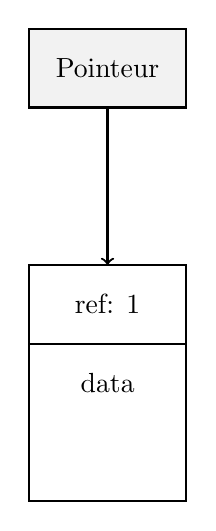
\begin{tikzpicture}[level distance=20mm,thick] 
    \draw (0,5) rectangle +(2,1) [fill=gray!10]  node[midway]
          {Pointeur};
          
    \draw (0,0) rectangle +(2,3)   node[midway]{data};
    \draw (0,2) rectangle +(2,1)   node[midway]{ref: 1};
    \draw[->] (1,5)--(1,3);
  \end{tikzpicture}
  \caption{}\label{cow1}
\end{subfigure}
\begin{subfigure}{.3\textwidth}
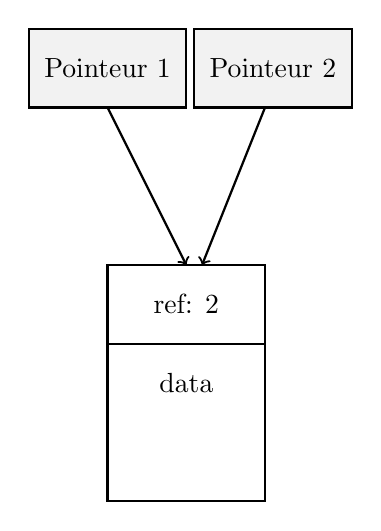
\begin{tikzpicture}[level distance=20mm,thick]
    \draw (0,5) rectangle +(2,1) [fill=gray!10]  node[midway]
          {Pointeur 1};
    \draw (2.1,5) rectangle +(2,1) [fill=gray!10]  node[midway]
          {Pointeur 2};      
    \draw (1,0) rectangle +(2,3)   node[midway]{data};
    \draw (1,2) rectangle (3,3)   node[midway]{ref: 2};
    \draw[->] (1,5)--(2,3);
    \draw[->] (3,5)--(2.2,3);
\end{tikzpicture}\caption{}\label{cow2}
\end{subfigure}
\begin{subfigure}{.3\textwidth}
  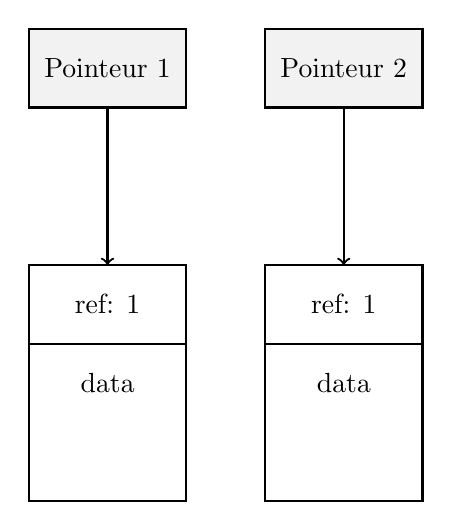
\begin{tikzpicture}[level distance=20mm,thick]
    \draw (1,5) rectangle +(2,1) [fill=gray!10]  node[midway]
          {Pointeur 1};
    \draw (4,5) rectangle +(2,1) [fill=gray!10]  node[midway]
          {Pointeur 2};
          
    \draw (1,0) rectangle (3,3)   node[midway]{data};
    \draw (1,2) rectangle (3,3)   node[midway]{ref: 1};
      
    \draw (4,0) rectangle (6,3)   node[midway]{data};
    \draw (4,2) rectangle (6,3)   node[midway]{ref: 1};
    
    \draw[->] (2,5)--(2,3);
    \draw[->] (5,5)--(5,3);
  \end{tikzpicture}\caption{}
  \label{cow3}
\end{subfigure}
\caption{Copy On Write}\label{cowall}
\end{figure}

\end{center}
